\documentclass[sigconf]{acmart}

\usepackage{listings}
\usepackage{booktabs}
\usepackage{graphicx}

% Copyright
%\setcopyright{none}
%\setcopyright{acmcopyright}
%\setcopyright{acmlicensed}
\setcopyright{rightsretained}
%\setcopyright{usgov}
%\setcopyright{usgovmixed}
%\setcopyright{cagov}
%\setcopyright{cagovmixed}

%% Comments
\newif\ifcomments\commentstrue

\ifcomments
\newcommand{\authornt}[3]{\textcolor{#1}{[#3 ---#2]}}
\newcommand{\todo}[1]{\textcolor{red}{[TODO: #1]}}
\else
\newcommand{\authornt}[3]{}
\newcommand{\todo}[1]{}
\fi

\newcommand{\ds}[1]{\authornt{red}{DS}{#1}} %Dan
\newcommand{\wss}[1]{\authornt{blue}{SS}{#1}} %Spencer
\newcommand{\jc}[1]{\authornt{magenta}{JC}{#1}} %Jacques
\newcommand{\spr}[1]{\authornt{green}{SP}{#1}} %Steven
\newcommand{\jtol}{$J_{\mbox{tol}}$}
\newcommand{\inlHask}[1]{\lstinline[language=Haskell, frame=single, showstringspaces=false]{#1}}
% DOI
%\acmDOI{10.475/123_4}

% ISBN
%\acmISBN{123-4567-24-567/08/06}

%Conference
\acmConference[SE-CSE\_SE-CoDeSE]{2017 International Workshop on Software Engineering
  for High Performance Computing in Computational and Data-Enabled Science and
  Engineering}{November 2017}{Denver, Colorado, USA} 
\acmYear{2017}
\copyrightyear{2017}

%\acmPrice{15.00}

\begin{document}
\title[Assembling Software from Knowledge]{GlassBR: Assembling well-documented software from a knowledge repository}
% \titlenote{Produces the permission block, and
%   copyright information}
% \subtitle{Extended Abstract}
% \subtitlenote{The full version of the author's guide is available as
%   \texttt{acmart.pdf} document}

\author{Daniel Szymczak}
% \authornote{Dr.~Trovato insisted his name be first.}
% \orcid{1234-5678-9012}
\affiliation{%
  \institution{Computing and Software Department, McMaster University}
  \streetaddress{1280 Main Street West}
  \city{Hamilton} 
  \state{Ontario} 
  \postcode{L8S 4K1}
}
\email{szymczdm@mcmaster.ca}

\author{Spencer Smith}
% \authornote{Dr.~Trovato insisted his name be first.}
% \orcid{1234-5678-9012}
\affiliation{%
  \institution{Computing and Software Department, McMaster University}
  \streetaddress{1280 Main Street West}
  \city{Hamilton} 
  \state{Ontario} 
  \postcode{L8S 4K1}
}
\email{smiths@mcmaster.ca}

\author{Jacques Carette}
% \authornote{Dr.~Trovato insisted his name be first.}
% \orcid{1234-5678-9012}
\affiliation{%
  \institution{Computing and Software Department, McMaster University}
  \streetaddress{1280 Main Street West}
  \city{Hamilton} 
  \state{Ontario} 
  \postcode{L8S 4K1}
}
\email{carette@mcmaster.ca}

\author{Steven Palmer}
%\authornote{The secretary disavows any knowledge of this author's actions.}
\affiliation{%
  \institution{Computing and Software Department, McMaster University}
  \streetaddress{1280 Main Street West}
  \city{Hamilton} 
  \state{Ontario} 
  \postcode{L8S 4K1}
}
\email{palmes4@mcmaster.ca}

% The default list of authors is too long for headers}
% \renewcommand{\shortauthors}{B. Trovato et al.}

\begin{abstract}

What if building well-documented software was not tedious and unrewarding?  We illustrate our Drasil framework through a worked example, GlassBR, of a piece of scientific software for computing the safety of glass panes with respect to explosions.  Such software is algorithmically straightforward, but as it is used in safety critical applications, correctness is important.  The setting we are most interested in is when correctness is judged via certification.

\end{abstract}

%
% The code below should be generated by the tool at
% http://dl.acm.org/ccs.cfm
% Please copy and paste the code instead of the example below. 
%
 \begin{CCSXML}
<ccs2012>
<concept>
<concept_id>10002950.10003705</concept_id>
<concept_desc>Mathematics of computing~Mathematical software</concept_desc>
<concept_significance>300</concept_significance>
</concept>
<concept>
<concept_id>10011007.10011074.10011092</concept_id>
<concept_desc>Software and its engineering~Software development techniques</concept_desc>
<concept_significance>300</concept_significance>
</concept>
<concept>
<concept_id>10011007.10011074.10011092.10011782</concept_id>
<concept_desc>Software and its engineering~Automatic programming</concept_desc>
<concept_significance>300</concept_significance>
</concept>
</ccs2012>
\end{CCSXML}

\ccsdesc[300]{Mathematics of computing~Mathematical software}
\ccsdesc[300]{Software and its engineering~Software development techniques}
\ccsdesc[300]{Software and its engineering~Automatic programming}

\keywords{scientific computing, software quality, software engineering, document
driven design, code generation}

\maketitle


\section{Introduction} \label{SecIntroduction}

Every developer should strive towards creating the highest possible quality 
software. This is especially true in safety-critical applications where incorrect software 
could cost lives. 

Our team is focused on improving the quality of Scientific Computing Software 
(SCS). We have chosen large, multi-year, multi-developer projects where the end 
users do much of the development as our target scope. For these projects, we pay 
particular attention to (re-)certifiability.

Certifying (or re-certifying) software can be lengthy and expensive with a 
single error causing the software to fail the certification process. We want to 
streamline the certification process, by simplifying the creation of the 
requisite software artifacts (documentation and code) for the certification 
process, and by ensuring that these artifacts are always consistent. Tracking 
down the source of any information contained in our artifacts should be 
trivially easy, yet this is not always the case as documentation is often not a 
high priority.

Often considered too high a cost in terms of time and effort for SCS developers, 
particularly when dealing with rapid changes in development, improved 
documentation is an important aspect of improving overall software quality and 
simplifying the certification process. Carver~\cite{CarverEtAl2007} observed 
that scientists do not view rigid, process-heavy approaches, favourably. 

Previous work by Smith \& Koothoor~\citep{SmithAndKoothoor2016} found 27 errors 
in an existing software project when creating new documentation. Any of these errors could have led to a failure in the certification process, had they been attempting to certify the software.

Developers are being made aware of the advantages of documentation~\cite{SmithJegatheesanAndKelly2016}, yet it can still be difficult to ensure it becomes a high priority because documenting software is typically felt to be:

\begin{itemize}
\item Too long
\item Too difficult to maintain
\item Not amenable to change
\item Too tied to the waterfall process
\item Counterproductive when reporting on each stage of 
		development~\citep{Roache1998}
\end{itemize}

There are also other issues with document-rich certifiable software development. Namely the vast amount of knowledge duplication across software artifacts. Consider a simple piece of software with the following artifacts:

\begin{itemize}
\item Software Requirements Specification (SRS)
\item Design Document
\item Source Code
\item Tests
\end{itemize}
Knowledge, such as the functional requirements, from the SRS is duplicated in both the source code and tests. That same knowledge appears in the design document as well, albeit in a transformed state. 

Now consider that software certification often requires a great many more artifacts than simply the four listed above. Much of the same knowledge will appear across all of the artifacts and will need to be maintained should anything change. Manually maintaining these artifacts is a lesson in tedium and the time spent, if it were easier to deal with duplication automatically, could be better used elsewhere.

With that in mind, how can we enjoy the benefits of documentation, without the usually
associated drudgery? Our proposed solution is \textit{Drasil} -- a framework that utilizes
a knowledge-based approach to software development, as originally proposed in a
position paper by Szymcak et al~\cite{SzymczakEtAl2016}. The goal of the
approach is to capture scientific and documentation knowledge in a reusable way,
then use that knowledge to generate the source code and all of the other software
artifacts (documentation, build files, tests, etc).

Several case studies have been reimplemented in Drasil over the course of the framework's development. In this paper we will focus on GlassBR, a piece of scientific software used in civil engineering for computing whether glass panes can safely withstand the force of explosions.

Work on Drasil has continued steadily since the original position paper, as
described below. We begin with a brief overview of the design of the Drasil
framework in Section~\ref{SecDesign}, then describe the development process that
has been adopted in Section~\ref{SecDevProcess}. Following this, we show an example of
Drasil in action (Section~\ref{SecGlassBR}) and the results we have seen to date
(Section~\ref{SecQuality}). Finally, we lay out some of the work that still
needs to be done (Section~\ref{SecFuture}) before concluding.

\section{Design of Drasil} \label{SecDesign}

Drasil's design is based around three main components:
\begin{enumerate}
	\item Knowledge capture mechanisms (\textit{Chunks})
	\item Artifact generation language(s) (\textit{Recipes})
	\item Knowledge-base (\textit{Data.Drasil})
\end{enumerate}

Chunks are the primary knowledge-capture mechanism. There are many flavours of 
chunks (as shown in Figure~\ref{hierarchy}). The most basic chunk is simply a 
piece of data with an id. From there, all other chunks can be created. For 
example, a \textit{Quantity} is a \textit{NamedIdea} (a chunk containing an id, 
as well as a term which represents the idea and a potential abbreviation for 
that term) which also has a \textit{Space} (integer, boolean, vector, etc.), 
and symbol representation/units (if applicable).  The notation in
Figure~\ref{hierarchy} uses a question mark (?) to indicate when a value may or
may not be present (Maybe types in Haskell).

\begin{figure}
	\centering
	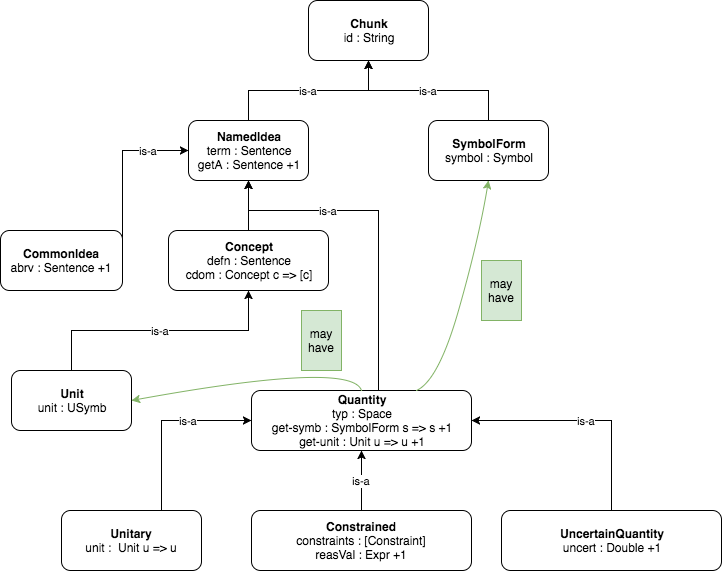
\includegraphics[width=0.5\textwidth]{figures/class_hierarchy.png}
	\caption{Drasil chunk hierarchy}
	\label{hierarchy}
\end{figure}

We can think of chunks as our building blocks of knowledge; they are the 
ingredients to be used in our \textit{Recipes}. Our language of recipes is a 
Domain-Specific Language (DSL) embedded in Haskell that is used to define what 
we would like to generate, and in what order. A small snippet of recipe 
language code for our Software Requirements Specification (SRS) can be seen in 
Figure~\ref{recipeLang}. This code is used to generate the \textit{Reference 
Materials} section of our SRS, which contains an introduction followed by the 
table of units, table of symbols, and table of abbreviations and acronyms 
subsections.

\begin{figure}
\begin{lstlisting}[language=Haskell, frame=single, showstringspaces=false, 
basicstyle=\small]
mkSRS :: DocDesc 
mkSRS = [RefSec (RefProg intro 
	[TUnits, 
	tsymb [TSPurpose, SymbOrder], 
	TAandA])]
        ...
\end{lstlisting}
\caption{The reference material section for an SRS written in Drasil's Document 
Language}
\label{recipeLang}
\end{figure}

The document generation language is highly abstracted, but allows for a fairly
high degree of customization. Drasil also contains a code-generation language
integrating GOOL~\cite{Costabile2012} -- a Generic Object-Oriented Language -- which can
generate code in a number of different target languages including Python, Lua,
and C++.  We will discuss code generation in more depth through the example in
Section~\ref{SecGlassBR}.

Finally, there is the knowledge-base for Drasil (located in Data.Drasil). We 
are creating a database of reusable scientific knowledge that can be applied 
across a number of different applications across multiple domains. As the 
Drasil framework grows, we hope to continue to expand this database into an 
ontology of scientific information for a number of disciplines. See 
Figure~\ref{ontology} for an example of some of the domains in which we have 
started to capture knowledge.

\begin{figure}
	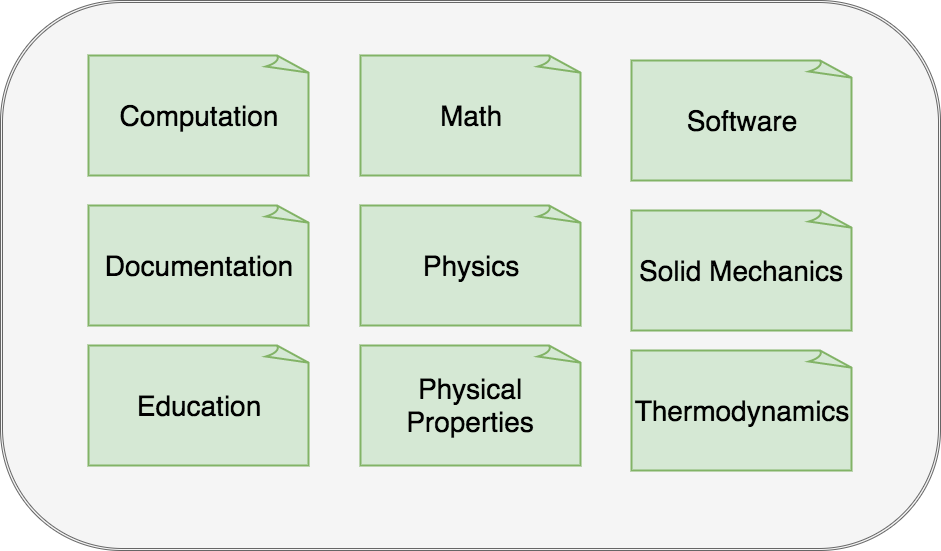
\includegraphics[width=.5\textwidth]{figures/ontology.png}
	\caption{Data.Drasil knowledge domains}
	\label{ontology}
\end{figure}

\section{Development Process for Drasil} \label{SecDevProcess}

Drasil is being developed using a practical, example-driven process. There are 
currently five different examples being developed concurrently within (and 
driving the development of) Drasil:

\begin{itemize}
\item Chipmunk2D Game Physics Engine
\item Solar Water Heating System Incorporating Phase Change Material (PCM)
\item Solar Water Heating System (No PCM)
\item Slope Stability Analysis
\item Glass Breakage Analysis (GlassBR)
\end{itemize}
The original (non-Drasil) documentation for these examples came out of a study
on Document Driven Design (DDD) for SCS~\cite{SmithJegatheesanAndKelly2016}.

Our practical design approach allows us the flexibility to prototype without 
over-designing. As a new feature becomes necessary to continue the 
implementation of a given example, only then do we design, test, implement, and 
re-test it. We occasionally implement features we may need in the future, but 
only in those instances when it is obvious that we are taking the right 
approach.

The five examples provided an ideal means to bring additional members on to the
project.  Summer student research assistants joined the project and were
responsible for completing most of the work on translating the original examples
into Drasil, and then later transforming the examples, as the Drasil DSLs have
been extended and refactored.  Through their work, the summer students have
demonstrated that using Drasil does not require prior knowledge of Haskell and
code generation techniques.  The student members of the Drasil project cover
disciplines ranging from Chemical Engineering, Applied Mathematics, Computer
Science and Software Engineering, with levels of education ranging from first to
third year. None of the students had prior knowledge of Haskell.

The current incarnation of the Drasil framework can be found on GitHub at 
\href{https://github.com/JacquesCarette/literate-scientific-software}
{https://github.com/JacquesCarette/literate-scientific-software}. We utilize 
peer-review of code throughout development to correct missteps early on, and 
keep an up-to-date issue tracker for any bugs, feature requests, or other 
``to-do'' tasks.

Progressive development of Drasil is achieved by not only looking for new 
features that must be implemented, but also through a cyclic approach towards 
improvement. This approach relies on finding new (extractable) patterns in the 
framework through refactoring, de-embedding and extracting knowledge from the 
example materials, and reducing knowledge duplication by capturing it in a 
highly reusable way.

By adopting a practical, example-driven, ``bottom-up,'' approach for the
development of Drasil, we have avoided the problems inherent in a more
theoretical, or ``top-down,'' approach.  The size, scope and complexity of SCS
means that attempting to imagine a priori the DSLs that we would need would be
exceedingly difficult.  We would invariably leave something out and likely
provide too simple a framework.  Rather than try to arbitrarily determine the
initial scope of Drasil, we let the examples tell us what they need. The
``bottom-up'' approach was previously successfully used for generating members
of the family of Gaussian elimination algorithms~\cite{Carette2006}.  

The idea that scientific software forms a program
family~\cite{SmithMcCutchanAndCao2007} is helpful for the current work.  We can
imagine that each of our five examples provides one specific instance of the
more general family of SCS.  With five examples we feel confident that enough of
the commonalities and variabilities between members of the family of SCS are
present that the initial implementation of Drasil will provide a reasonable
starting point for implementing a representative subset of the full family of
SCS.

\section{A Practical Example (GlassBR)} \label{SecGlassBR}

GlassBR is a piece of software used in Civil Engineering to predict whether or 
not a slab of glass will be able to withstand a given blast without breaking. It
has two classes of input: glass geometry and blast type. Each of these input 
classes has a number of fields (glass type, dimensions, TNT equivalent factor, 
standoff distance, etc.) used as input to the simulation. Also, a tolerable 
probability of breakage is given by the user.

The output of GlassBR is whether or not the glass slab is considered safe. This 
is based on a probability that is calculated through interpolation being 
compared to the tolerable probability.

To understand the Drasil implementation, we will follow one specific piece of 
knowledge through from requirements to code. We intend to show how this 
knowledge is captured and used in Drasil to produce our software artifacts 
(documentation and code).


%- bottom up approach to presentation - start with chunks, build up to SRS, traceability

\begin{figure}
\begin{center}
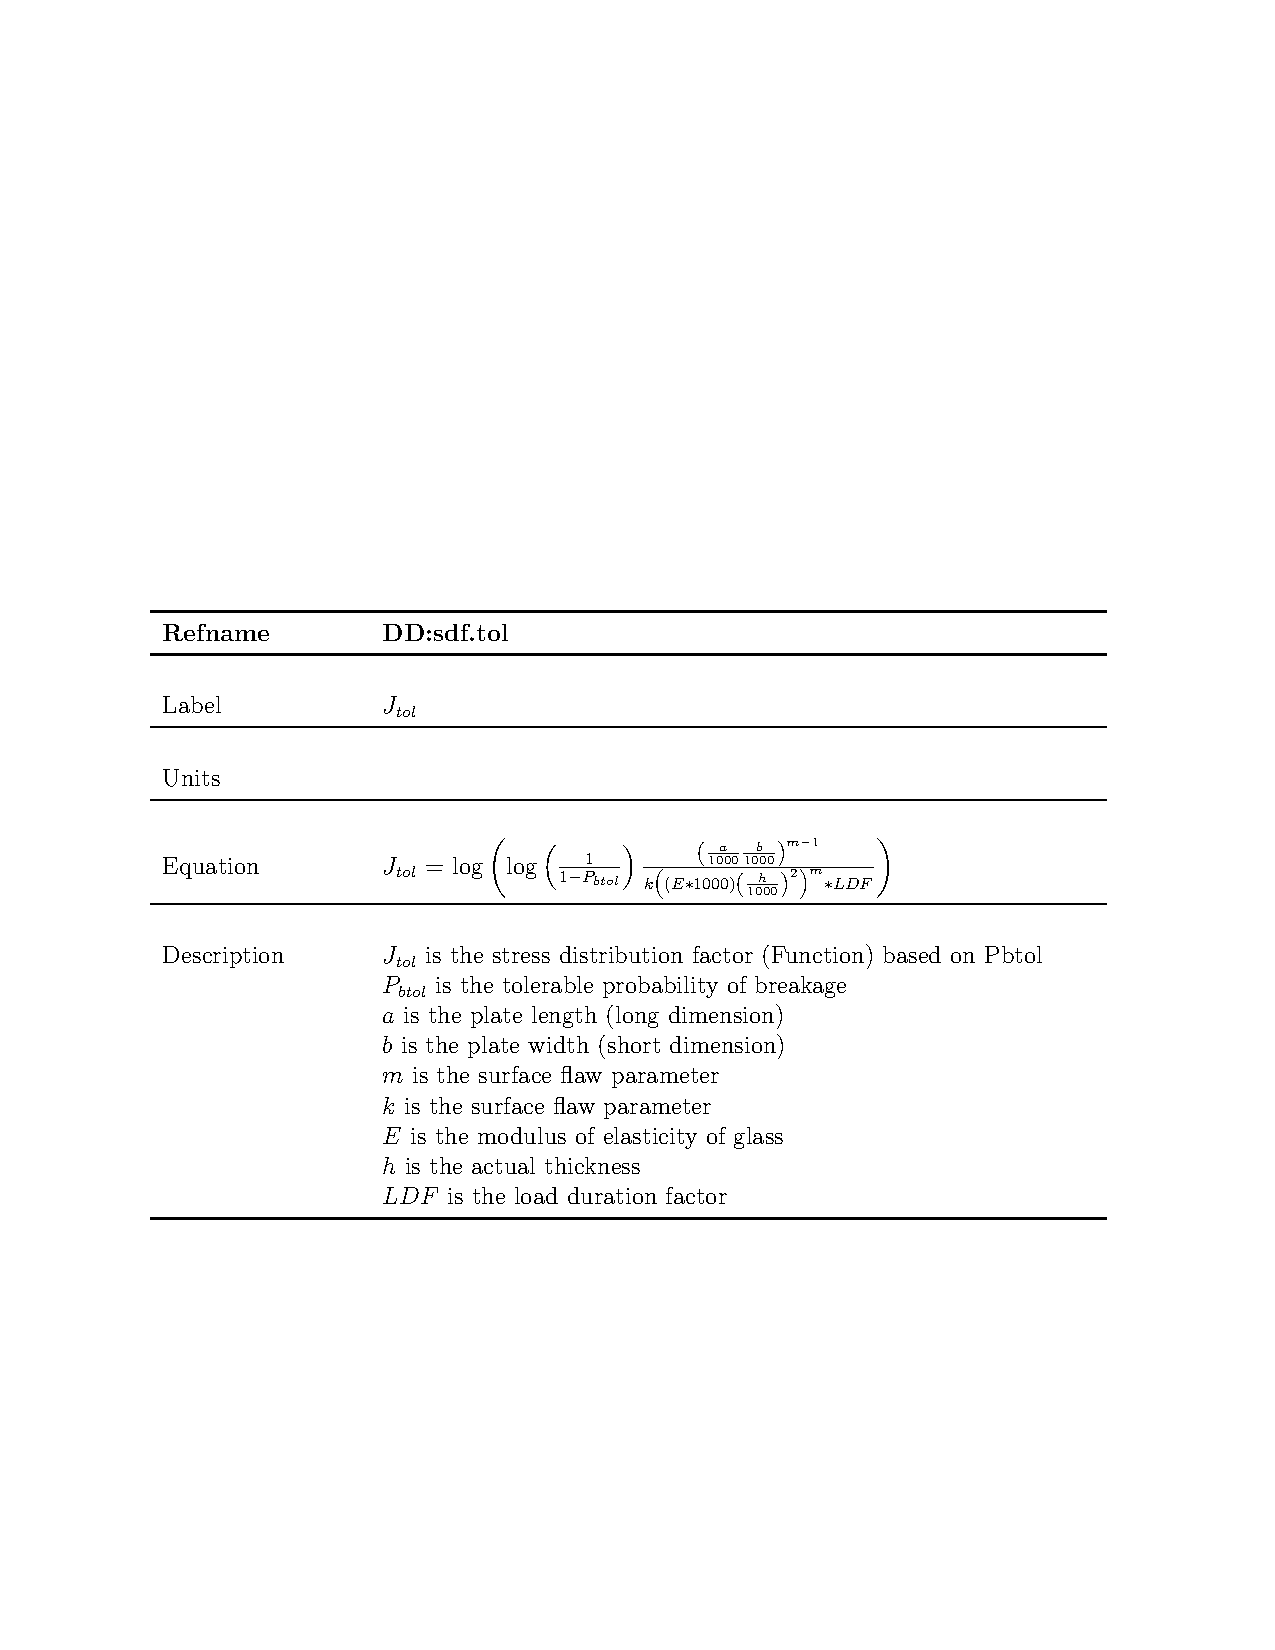
\includegraphics[width=0.45\textwidth]{./figures/Jtol_pdf.pdf}
\end{center}
\caption{\jtol{} from GlassBR Requirements}
\label{Fig_Jtolpdf}
\end{figure}

Let us start by taking a look at a data definition for the tolerable stress 
distribution factor (\jtol{}) from GlassBR. Figure~\ref{Fig_Jtolpdf} 
shows the Drasil-generated TeX version of the data definition for 
\jtol{}, however we can also generate the documents in HTML. This 
figure is part of the requirements for the GlassBR software, and as such, we 
will eventually need code (like that in Figure~\ref{Fig_JtolPython}) that can be
used to calculate \jtol{}. We can generate this code as well! Not only 
that, but thanks to the incorporation of GOOL we can also generate Java, Lua, 
etc. 

\begin{figure*}
\begin{lstlisting}[language=python, frame=single, showstringspaces=false, 
basicstyle=\small]
def calc_j_tol(inparams):
    j_tol = math.log((math.log(1.0/(1.0 - inparams.pbtol))) * ((((inparams.a / 1000.0) * 
        (inparams.b / 1000.0)) ** (inparams.m - 1.0)) / ((inparams.k * (((inparams.E * 1000.0) * 
        ((inparams.h / 1000.0) ** 2.0)) ** inparams.m)) * inparams.ldf))) 
    return j_tol
\end{lstlisting}
\caption{Python code to Calculate \jtol{}}
\label{Fig_JtolPython}
\end{figure*}

The source knowledge for generating both the documentation and the code has been
captured using chunks as shown in Figure~\ref{Fig_JtolDrasil}. The value of 
\jtol{} is calculated from the expression {\inlHask{tolStrDisFac_eq}}, which is 
part of the {\inlHask{tolStrDisFac}} chunk.

\begin{figure*}
\begin{lstlisting}[language=Haskell, frame=single, showstringspaces=false, 
basicstyle=\small] 
stressDistFac = makeVC "stressDistFac" (nounPhraseSP $ "stress distribution" ++ " factor (Function)") cJ

sdf_tol = makeVC "sdf_tol" (nounPhraseSP $ "stress distribution" ++ " factor (Function) based on Pbtol") 
  (sub (stressDistFac ^. symbol) (Atomic "tol"))

tolStrDisFac_eq :: Expr
tolStrDisFac_eq = log (log ((1) / ((1) - (C pb_tol))) * ((Grouping (((C plate_len) / (1000)) * 
  ((C plate_width) / (1000)))) :^ ((C sflawParamM) - (1)) / ((C sflawParamK) * 
  (Grouping (Grouping ((C mod_elas) * (1000)) * (square (Grouping ((C act_thick) / (1000)))))) :^ 
  (C sflawParamM) * (C loadDF))))

tolStrDisFac :: QDefinition
tolStrDisFac = mkDataDef sdf_tol tolStrDisFac_eq
\end{lstlisting}
\caption{Drasil (Haskell) code for \jtol{} Knowledge}
\label{Fig_JtolDrasil}
\end{figure*}

Notice there is actually an error in the code and documentation. We should not 
be dividing by 1000 in a number of places. Luckily, with one quick change to 
{\inlHask{tolStrDisFac_eq}} (shown in Figure~\ref{Fig_JtolDrasil_fix}), we have 
corrected the error in our knowledge-base. Thus, after re-running the generator,
our code and documentation has now been fixed and remains consistent.

\begin{figure*}
\begin{lstlisting}[language=Haskell, frame=single, showstringspaces=false, 
basicstyle=\small]
tolStrDisFac_eq :: Expr
tolStrDisFac_eq = log (log ((1) / ((1) - (C pb_tol))) * ((Grouping ((C plate_len) * (C plate_width))) :^
  ((C sflawParamM) - (1)) / ((C sflawParamK) * (Grouping ((C mod_elas) * (square (C act_thick)))) :^ 
  (C sflawParamM) * (C loadDF))))
\end{lstlisting}
\caption{Modified Drasil (Haskell) code for \jtol{}}
\label{Fig_JtolDrasil_fix}
\end{figure*}

We have similarly captured all of the knowledge pertaining to GlassBR in chunks.
This knowledge can be assembled and extracted in different ways to produce a 
multitude of views, i.e. our artifacts, including the SRS. For a sense of what 
we can generate from this knowledge, see the table of contents for the currently
generated GlassBR SRS (Figure~\ref{Fig_ToCGlassBRSRS}). Again, our documents can
be generated in TeX and/or HTML for more flexibility. Both contain automated 
internal references.

\begin{figure}
\begin{center}
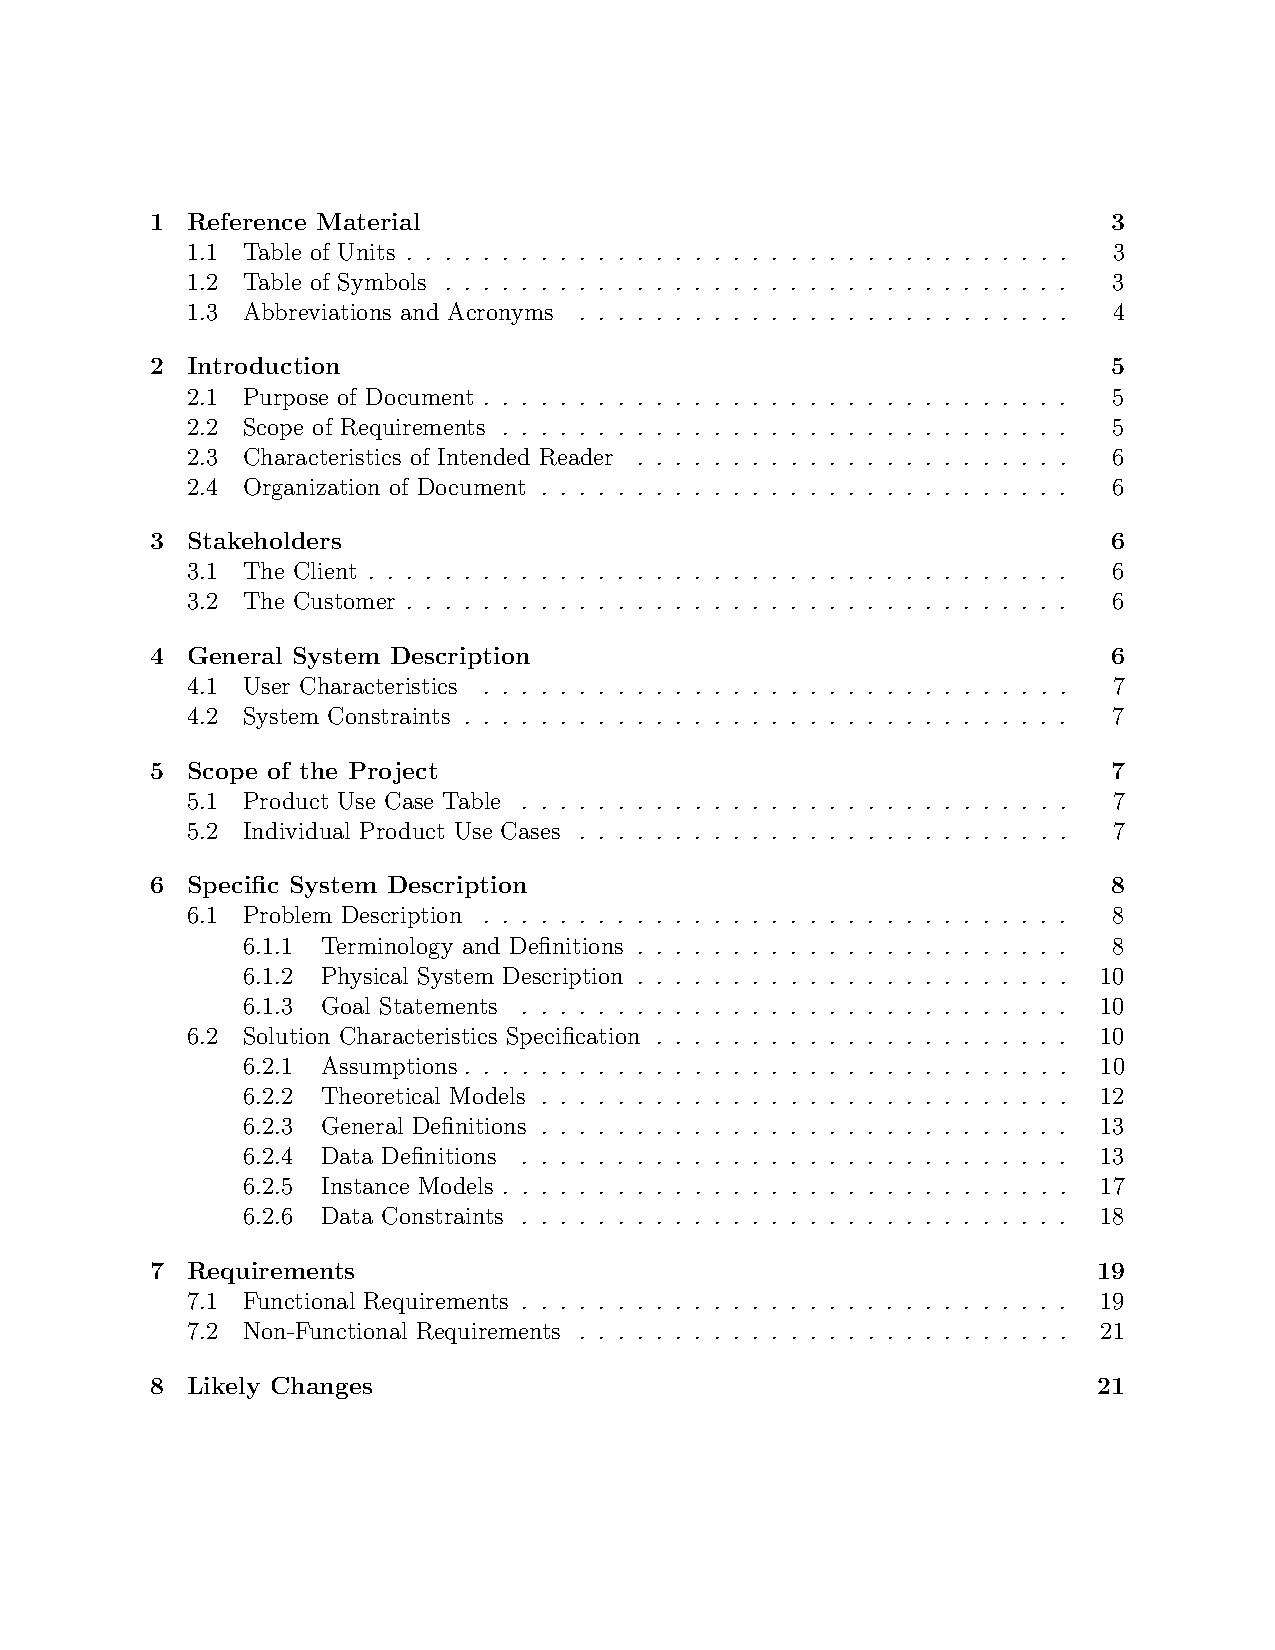
\includegraphics[scale=0.5]{./figures/TofC.pdf}
\end{center}
\caption{Table of Contents for Generated SRS for GlassBR}
\label{Fig_ToCGlassBRSRS}
\end{figure}

Another thing to note in our SRS is that the traceability information between
definitions, assumptions, theories, and instance models is automatically 
generated, including the traceability graph shown in 
Figure~\ref{Fig_TraceGraph}.

\begin{figure}
\begin{center}
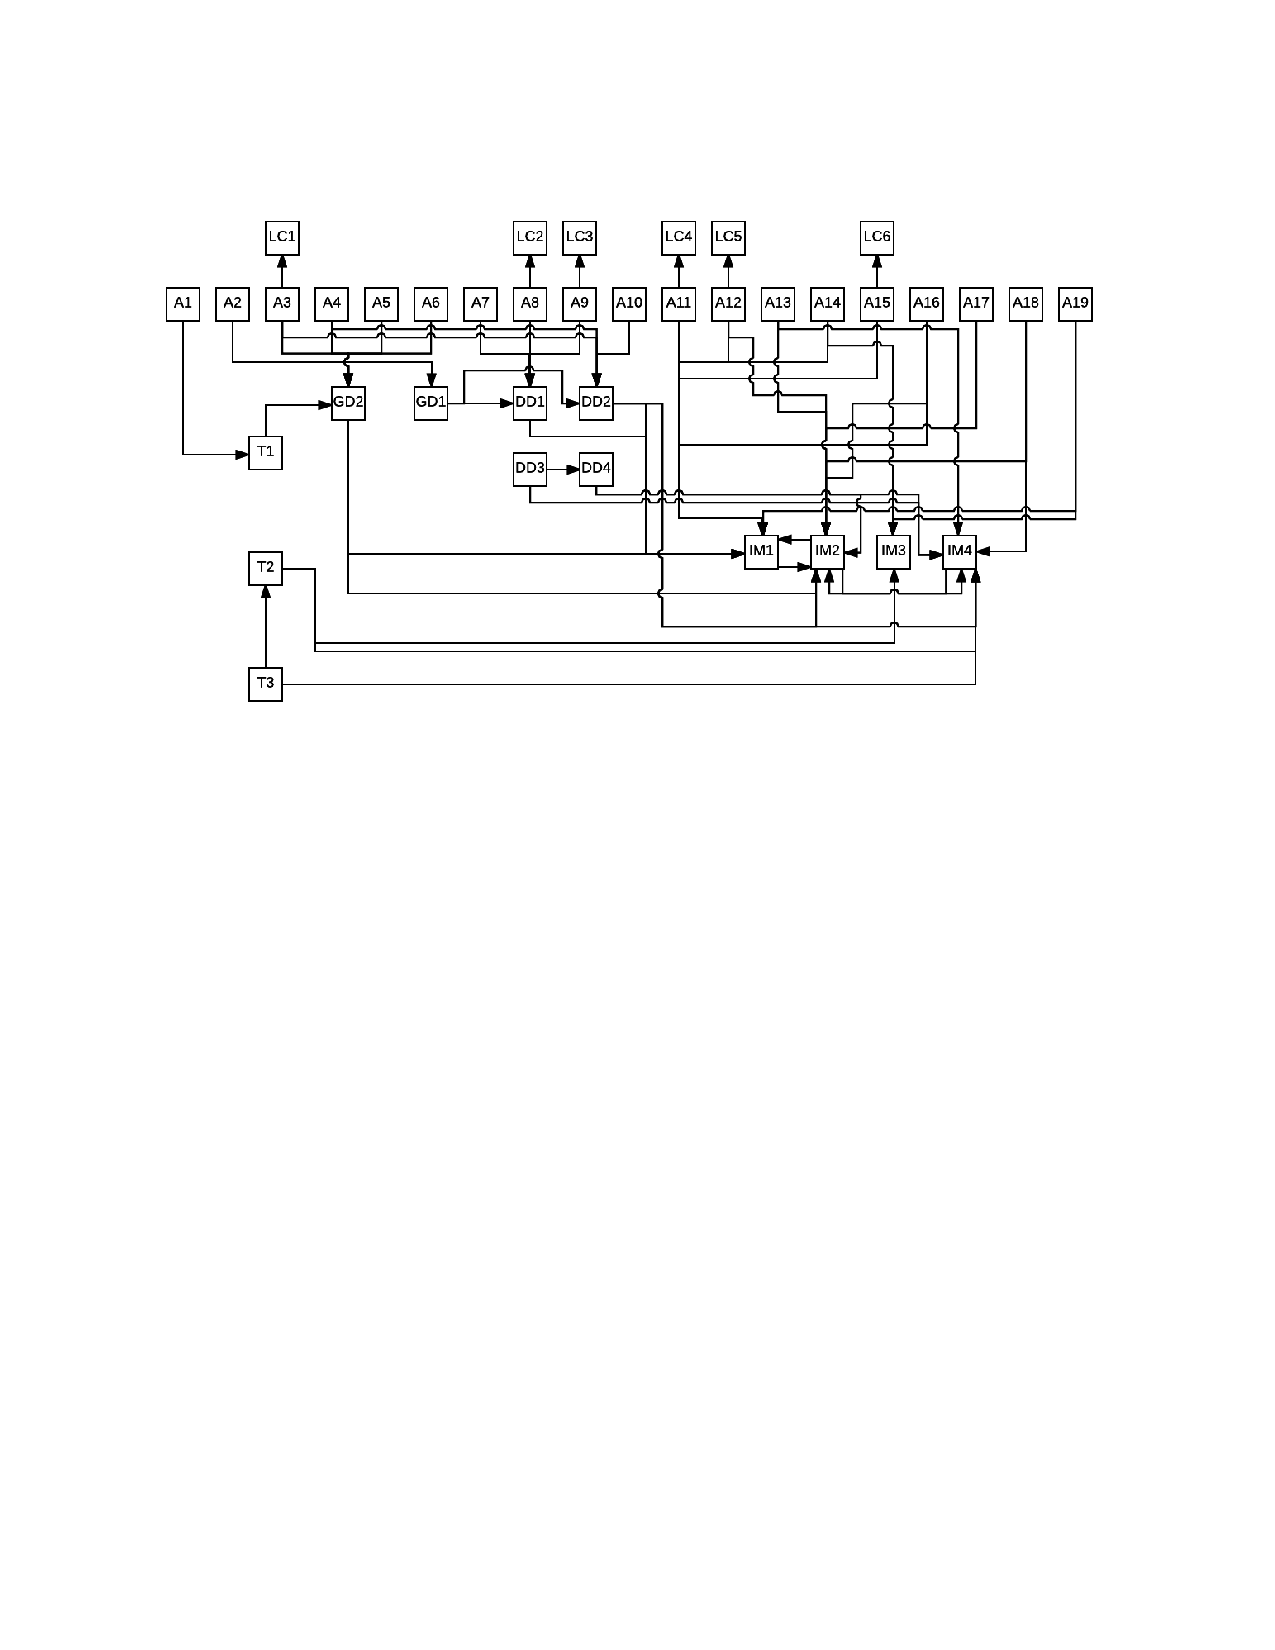
\includegraphics[scale=0.5]{./figures/TraceGraph.pdf}
\end{center}
\caption{Traceability Graph}
\label{Fig_TraceGraph}
\end{figure}

\section{Quality Improvements} \label{SecQuality}

Throughout Drasil's development lifecycle, we have already noticed a number of 
non-trivial quality improvements to the software examples being re-developed. 
These improvements come in a wide range of areas, but for the sake of brevity 
we will focus on certifiability, reusability, and reproducibility.

\subsection{Certifiability}

Certifying (or re-certifying) software can be a lengthy and expensive process 
where a single error can cause the software to fail the certification process. 
Consider the following equation from our solar water heating example which 
states that energy must be conserved:

\begin{equation*}
E_W = \int_{0}^{t} h_C A_C (T_C - T_W(t)) dt - \int_{0}^{t} h_P A_P (T_W(t) - T_P(t)) dt
\end{equation*}

This is trivial for a human to check, and writing code to check it during the 
software execution is also very simple. However, it is still time-consuming and 
should it ever need to change, it would require developers to make a number of 
modifications to many artifacts  in the future.

\begin{table} 
\centering
\caption{Constraints on Quantities -- Used To Verify Inputs}
\begin{tabular}{c c r c } 
\toprule
\textbf{Var} & \textbf{Constraints} & \textbf{Typical Value} & \textbf{Uncertainty}\\ \midrule
$L$ & $L > 0$ & 1.5 m & 10\% \\ 
$\rho_P$ & $\rho_P > 0$	& 1007 kg/m$^3$	& 10\% \\
\bottomrule
\end{tabular}
\label{tab:pcm}
\end{table}

Thanks to Drasil's knowledge-capture mechanisms, we can capture the above 
equation in one place, thus any changes can be made very quickly. Not only 
that, but sanity checks (such as ensuring constraints on inputs) can also be 
captured and reused (see Table~\ref{tab:pcm}). Capturing that information also 
delivers a wider array of advantages, including:

\begin{itemize}
\item Generate guards against invalid input automatically
\item Generate certain test cases automatically
\item Generate views suitable for inspection
\end{itemize}
We can also see that it is extremely easy to trace changes and verify that they 
are correct, thanks to our one-source, generative approach. We can produce 
documents similar to those commonly found in literate programming where we 
display the equations and code implementations (example: the \jtol{} equation 
and the python code used to calculate it) side-by-side, allowing a human to 
quickly verify the code is correct.

We have also touched on one of the greatest advantages which was implied 
earlier: \emph{If there is an error somewhere, it is wrong everywhere}. This 
may seem like a disadvantage, but ensuring every artifact contains the same 
errors means there is a much greater chance of those errors being spotted. In 
our experience, many examples of software include code that does not match the 
design (due to hacks, last-minute changes, etc.), and an error which could 
hamper certification efforts can fly under the radar. 

For (re-)certification purposes, we want to be able to find any and all errors, 
trace them to their source, and fix them quickly. Drasil has shown great 
promise in that respect.

\subsection{Reusability}

Reusability is a core tenet of ours for Drasil's development. This can be seen 
most obviously in the knowledge-capture mechanisms we have created. 

Consider the following software artifacts typically found in a rational, design 
process for software development~\cite{ParnasAndClements1986}:

\begin{itemize}
\item Software Requirements Specification (SRS)
\item Module Interface Guide (MIS)
\item Source Code
\item Test cases
\end{itemize}

Within these artifacts, there is a lot of duplication of specific knowledge 
related to the software being designed. Knowledge from the SRS will appear, 
possibly transformed, throughout each of the other artifacts. We seek to 
de-embed specific knowledge from within any specific artifact to easily reuse 
it throughout them all. This knowledge includes, but is not limited to:

\begin{itemize}
\item Scientific Knowledge
\item Models
\item Units
\item Symbols
\item Descriptions
\item Traceability information
\end{itemize}

\ds{TODO: Something about Drasil being awesome at capturing info.}

Reusing knowledge across artifacts in one software project is already 
incredibly useful, however, we have taken it a step further. Drasil allows us 
to reuse between projects. We can reuse a family of related models, or reuse 
pieces of knowledge from a given domain as necessary. Consider the vast number 
of software that rely on interpolation, or must ensure conservation of thermal 
energy. We can capture this knowledge once and reuse it through all of these 
projects.

We have already begun using knowledge across projects with great results. Our 
two implementations of the solar water heating systems have a vast amount of 
overlap in the requisite knowledge, except for the phase change material, which 
is not present in one of the examples.

\subsection{Reproducibility}

Typically when we refer to reproducibility the emphasis is on reproducing code 
execution. There are many problems attaining reproducibility at that 
level~\cite{IonescuAndJansson2013} as there are often undocumented:

\begin{itemize}
\item Assumptions
\item Modifications
\item Hacks
\end{itemize}

This does not mean that it is impossible to reproduce the execution of some 
given code, however, what if that code is wrong? Should it not be easier to 
independently replicate the work of others without relying on the code they've 
written?

We want to replicate not only the execution of the code, but the whole of the 
software from theory to implementation. Given the appropriate theoretical 
knowledge, assumptions, equations, etc. we should be able to take this 
high-level knowledge and reproduce an implementation which will return 
consistent results. Drasil allows us to do exactly this; we can capture the 
high-level science knowledge and use it to reproduce a piece of software. We 
can also package our projects in a Drasil-ready format, such that the software 
can be generated on-the-fly by any who wish to replicate the results or 
double-check the science.

Drasil can also potentially check for completeness and consistency, ensuring 
the little things that are tedious (if trivial) to manually verify. For 
example: every symbol should be defined and used and should not change 
throughout the artifacts (inter- and itra-artifact consistency). This may seem 
minor, but one of our case studies, which had been reviewed by humans on 
numerous occassions, introduced a new symbol for an existing concept in an 
equation derivation which was never defined and did not appear in the table of 
symbols. When implementing the project in Drasil, however, this error was made 
obvious almost immediately.

Overall, Drasil lends itself incredibly well to ensuring reproducibility in a 
much larger sense than we normally consider. It allows us to focus on the 
science, building our projects from the fundamental knowledge instead of 
relying on a lone developer's code.

\section{Future Work} \label{SecFuture}

Drasil has come a long way in the last year, yet there is still much to be 
done. With the current code-generation mechanisms being fairly naive, we have 
begun work on a language of design which allows us to apply design decisions to 
the theory knowledge to produce more flexible code. This language allows us to 
classify design and implementation choices in a reusable manner and will 
allow us to progress with the generation of design documents, which are 
currently difficult to produce in Drasil.

Another large feature that will be a necessity in the long-run, but has thus 
far been relegated to the back-burner, is a much more user-friendly syntax, or 
even a tool to aid in the creation of Drasil documents. Currently, Drasil is 
fairly arcane to use, even with our inclusion of more documentation. Yet, with 
each iteration of the language we introduce new, simplifying abstractions, 
which have already made it easier to use. However, we are aware of the gap that 
needs to be closed before it will be ready for our target users.

We are also continuing work on:
\begin{itemize}
	\item Generating new types of software artifacts
	\item Implementing much larger examples
\end{itemize}

Thanks to our practical-approach to Drasil's design, there will likely be many 
other minor features to add and changes to make that are not yet entirely clear 
to us.

\section{Concluding Remarks}

While Drasil is still a work-in-progress, it shows great promise as a tool to 
aid SCS developers. The ability to capture scientific knowledge, document it, 
and transform it into usable code from a single, fully-traceable source should 
not be underestimated.

We have already seen non-trivial improvements to existing software during its 
re-implementation in our current working-copy of Drasil. The case studies are 
now easier to verify, maintain, reuse, and replicate than they were before. 
There is also far less ambiguity on where certain concepts originated, as 
everything is captured in one source.

Not only will scientists be able to create higher quality software; they will 
be able to replicate and reuse each other's work in a far more robust manner 
than we have currently seen in practice. We hope Drasil will solve many of the 
reproducibility problems mentioned by Ionescu and 
Jansson~\cite{IonescuAndJansson2013}.

Software (re-)certification will also become a far less daunting task in a
future with Drasil. With full traceability of information and the ability to 
generate new document views on-the-fly, we will be able to streamline the 
process.

While developing in Drasil does come with a fairly high up-front investment, we 
believe the long-term maintainability along with the streamlining of 
verification/certification and other previously mentioned advantages 
will be well worth the cost.

\begin{acks}
The assistance of McMaster University's Dr.\ Manuel Campidelli, Dr.\ Wael and
Dr.\ Michael Tait with the GlassBR example is greatly appreciated.
\end{acks}

\bibliographystyle{ACM-Reference-Format}
\bibliography{SzymczakEtAl2017} 

\end{document}